\chapter{Background}
\label{chap:background}

This section defines the important aspects of timed automata and briefly
explains the reachability algorithm presented in
\cite{bengtsson2004timed} and demonstrates it on some examples (based on examples, also from \cite{bengtsson2004timed}).
%The verification of Fischer's protocol is presented as an example. 
CEGAR is also explained at a high level.


\section{Basic Definitions}
A \emph{valuation} $v(\mathcal{C})$ assigns a non-negative real value
to each clock variable $c \in \mathcal{C}$, where $\mathcal{C}$ denotes the set of clock
variables. For bravity, the term \emph{clock} is used as a synonym of {clock variable}.

A \emph{clock constraint} is a conjunctive formula of atomic
constraints of the form $x \sim n$ or $x - y \sim n$ (\emph{difference
	constraint}), where $x,y \in \mathcal{C}$ are clock variables, $\sim \in
\{\leq,<,=,>,\geq\}$ and \hbox{$n \in \mathbb{N}$}. $\mathcal{B}(\mathcal{C})$ represents the set of clock
constraints.

A \emph{timed automaton} $\mathcal{A}$ is a tuple $\langle L, l_0,
E, I\rangle$ where
$L$ is the set of locations,
$l_0 \in L$ is the initial location,
$E \subseteq L \times \mathcal{B}(\mathcal{C}) \times 2^\mathcal{C} \times L$
is the set of edges and,
$I: L \to \mathcal{B}(\mathcal{C})$ assigns invariants to locations.  Invariants can be used to ensure the progress of time in the model.


A state of $\mathcal{A}$ is a pair $\langle l,v \rangle$ where $l \in L$ is a
location and $v$ is the current valuation satisfying $I(l)$. In the initial
state $\langle l_0,v_0 \rangle$ $v_0$ assigns 0 to each clock variable.

Two kinds of operations are defined. The state $\langle l,v \rangle$ has a
\emph{discrete transition} to $\langle l',v' \rangle$  if there is an
edge $e(l,g,r,l') \in E$ in the automaton such that $v$ satisfies $g$, $v'$ assigns 0 to any $c \in
r$ and assigns $v(c)$ otherwise and $v'$ satisfies $I(l')$. The state $\langle
l,v \rangle$ has a \emph{time transition} to $\langle l,v' \rangle$ if $v'$
assigns $v(c)+d$ for some non-negative $d$ to each $c \in \mathcal{C}$ and $v'$
satisfies $I(l)$. 


\section{Reachability Analysis} \label{sec:reach}  

A \emph{zone} is a set of nonnegative clock valuations satisfying a set of clock constraints.
The set of all valuations reachable from a zone $z$ by time transitions is denoted by $z^\uparrow$.

A \emph{zone graph} is a finite graph consisting of $\langle l,z \rangle$ pairs as nodes, where $l \in L$ refers to some
location of a timed automaton and $z$ is a zone. Therefore, a node denotes a set
of states. Edges between nodes denote transitions. 

The construction of the graph starts with the initial node  $\langle l_0,z_0 \rangle$,
where $l_0$ is the initial location and $z_0$ contains the valuations reachable in the initial location by time transition. 
Next, for each outgoing edge $e$ of the initial location (in the automaton) a new node  $\langle l,z \rangle$ is created (in the zone graph) with an edge
$\langle l_0,z_0 \rangle \to \langle l,z \rangle$, where $\langle l,z \rangle$ contains the states to which the states in $\langle l_0,z_0 \rangle$ have a discrete transition through $e$. Afterwards $z$ is replaced by $z^\uparrow$.  The procedure is repeated on every newly introduced node of the zone graph. If the states defined by a newly introduced node $\langle l,z \rangle$ are all contained in an already existing node $\langle l,z' \rangle$, $\langle l,z \rangle$ can be removed, and the incoming edge should be redirected to $\langle l,z' \rangle$.

\begin{figure}
	\centering
		\begin{minipage}[c] {0.25\linewidth}%
	%		\vspace*{1pt}%
		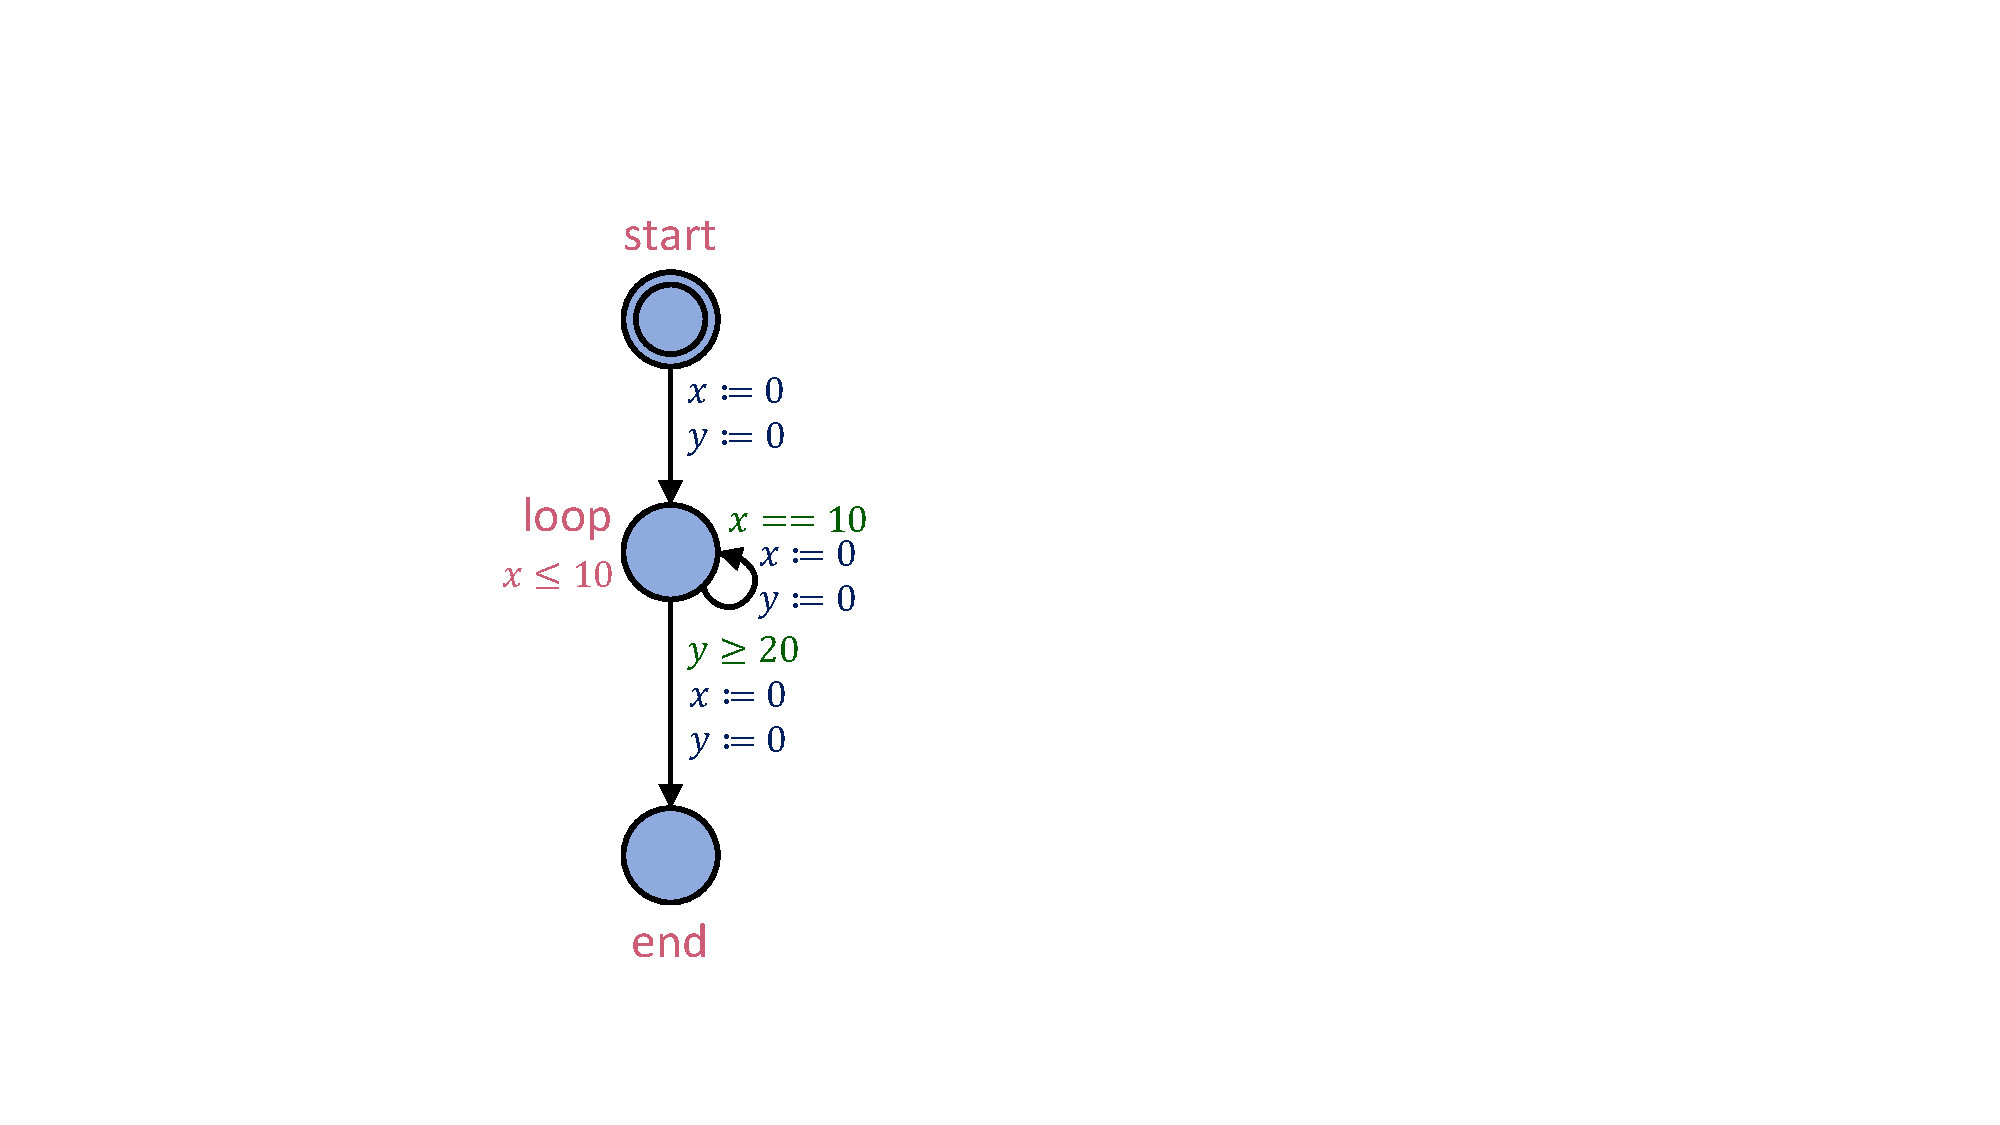
\includegraphics [width=\textwidth]{include/figures/loop_example_finite}%
		%\caption{Example of a timed automaton}
		\label{fig:loopfinite}
		\end{minipage}%
	%	%
		\begin{minipage}[c] {0.25\linewidth}%
			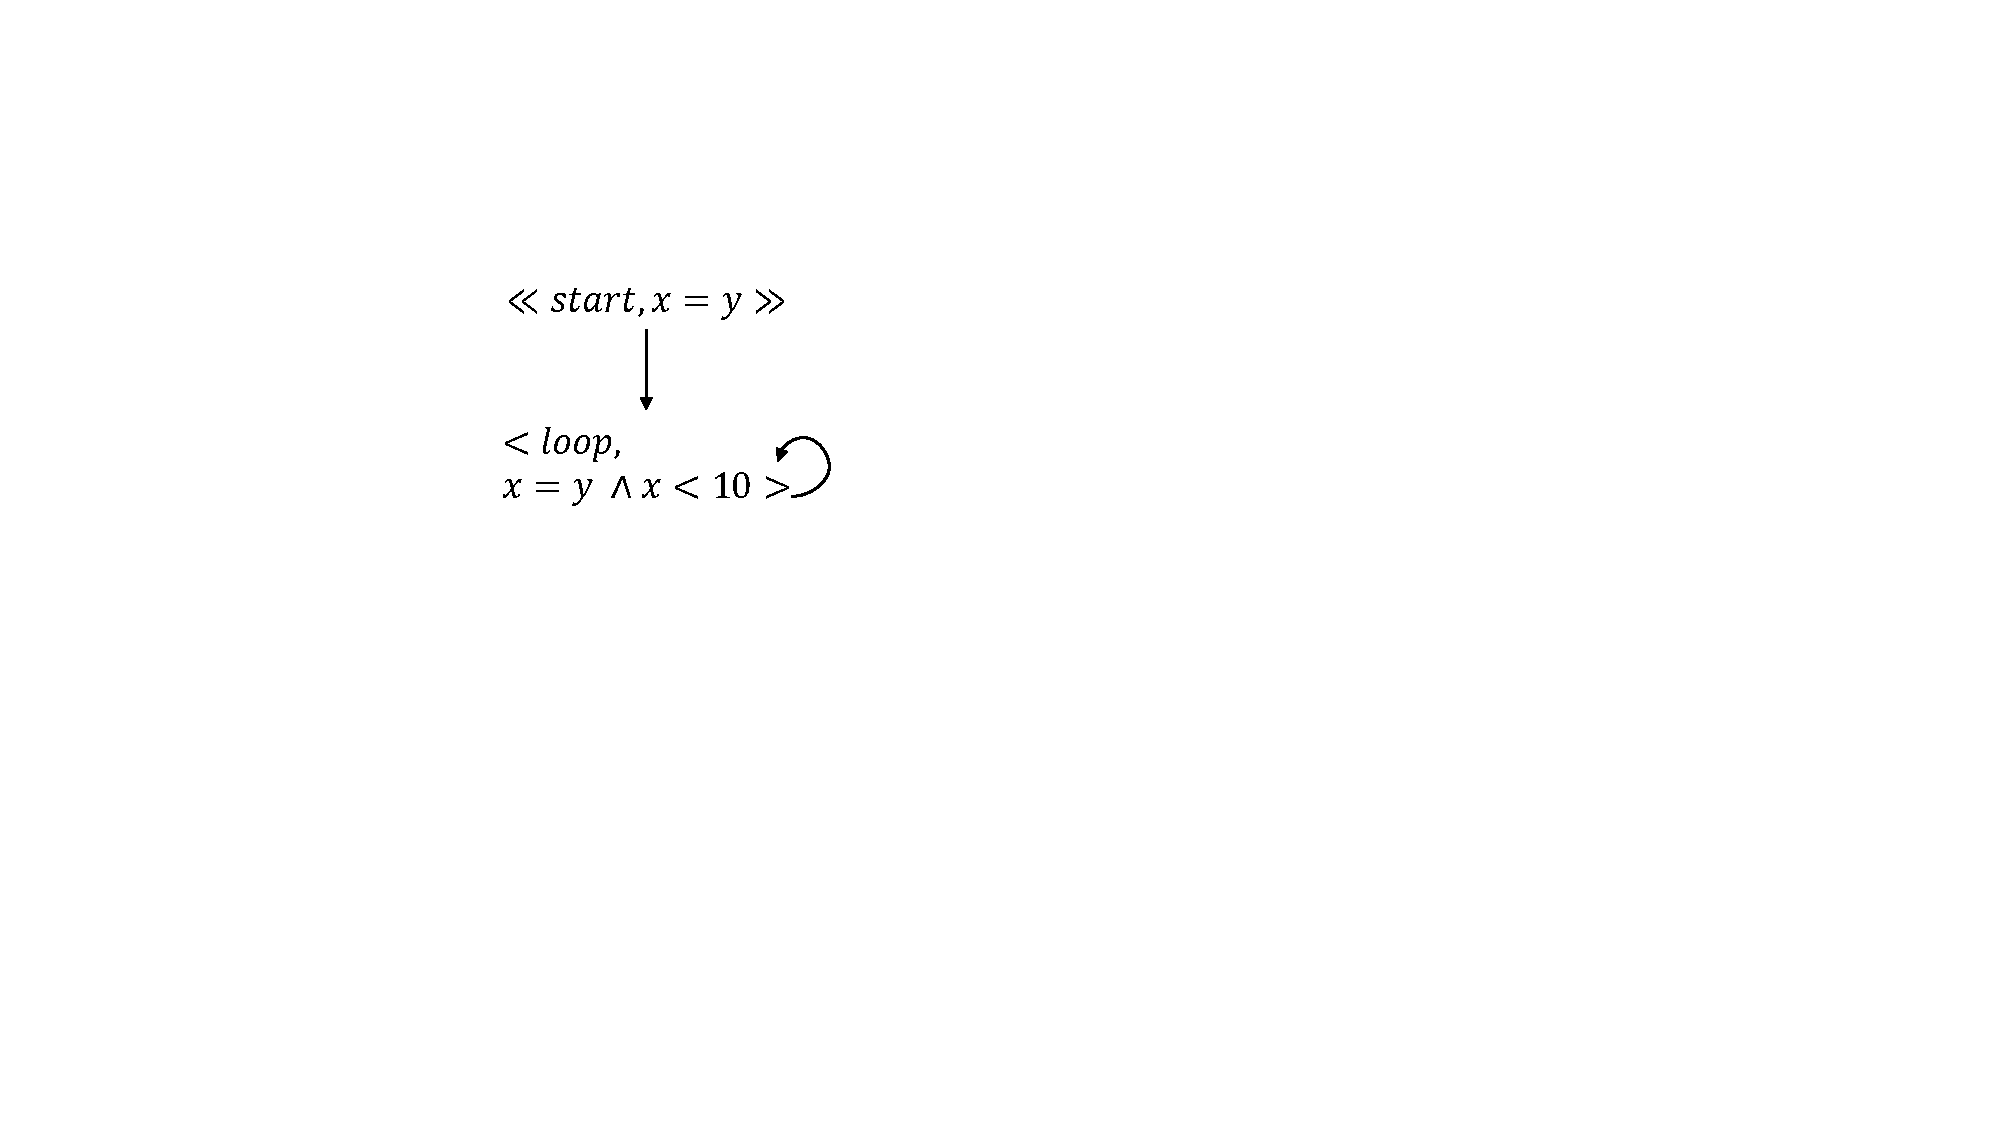
\includegraphics [width=\textwidth] {include/figures/loop_finite_zonegraph}%
	%		\vspace*{4pt}%
	%		\caption{Timed automaton}
			\label{fig:loopfinitegraph}
		\end{minipage}
	\caption{Timed automaton and it's zone graph}
\end{figure}  

%\todo{Example környezet}
\begin{example}
	


For ease of understanding the algorithm is demonstrated on the automaton on Figure \ref{fig:loopfinite}. The inital state is  $\langle start, z_0 \rangle$ where $z_0$ is a zone containing only te initial valuation $v_0(x)=0, v_0(y)=0$. The initial node is  $\langle start, z_0^\uparrow  \rangle$, where $z_0^\uparrow$ contains all states reachable form the initial state by delay. Since as time passes, the values of the two clocks will be incremented by the same value, $x$ and $y$ has the same value in each valuation contained by $z_0^\uparrow$. Since there is no invariant in location $start$ $x$ and $y$ can take any positive value. Because of this $z_0$ can be defined by the constraint $x=y$ (that is, $x-y = 0$), and the initial node can be defined as $\langle start; x=y  \rangle$.

There is only one outgoing transition from location $start$ and that resets $x$ and $y$ both, resulting in the same zone $z_0$ like before. The invariant $x \leq 10$ of location $loop$ is satisfied by $z_0$, but we have to consider it when calculating the valuations reachable by delay - only the states satisfying $x \leq 10$ of $z_0^\uparrow$ are reachable. The node of the graph can be defined as $\langle loop, x=y \wedge x<10 \rangle$.

There are two outgoing transitions from this node. The loop transition resets the clocks resulting in $z_0$ again in node $loop$. From this we know that instead of creating a new node in the graph, this time we only have to create a loop-edge from the last node.

Since there is no state in $\langle loop, x=y \wedge x<10 \rangle$ where $y \geq 20$ holds, the last transition will never be enabled, the zone graph is finished.
 The result can be seen on Figure \ref{fig:loopfinitegraph}.

\end{example}

\begin{figure}
	\centering
	\begin{minipage}[c] {0.25\linewidth}%
		%		\vspace*{1pt}%
		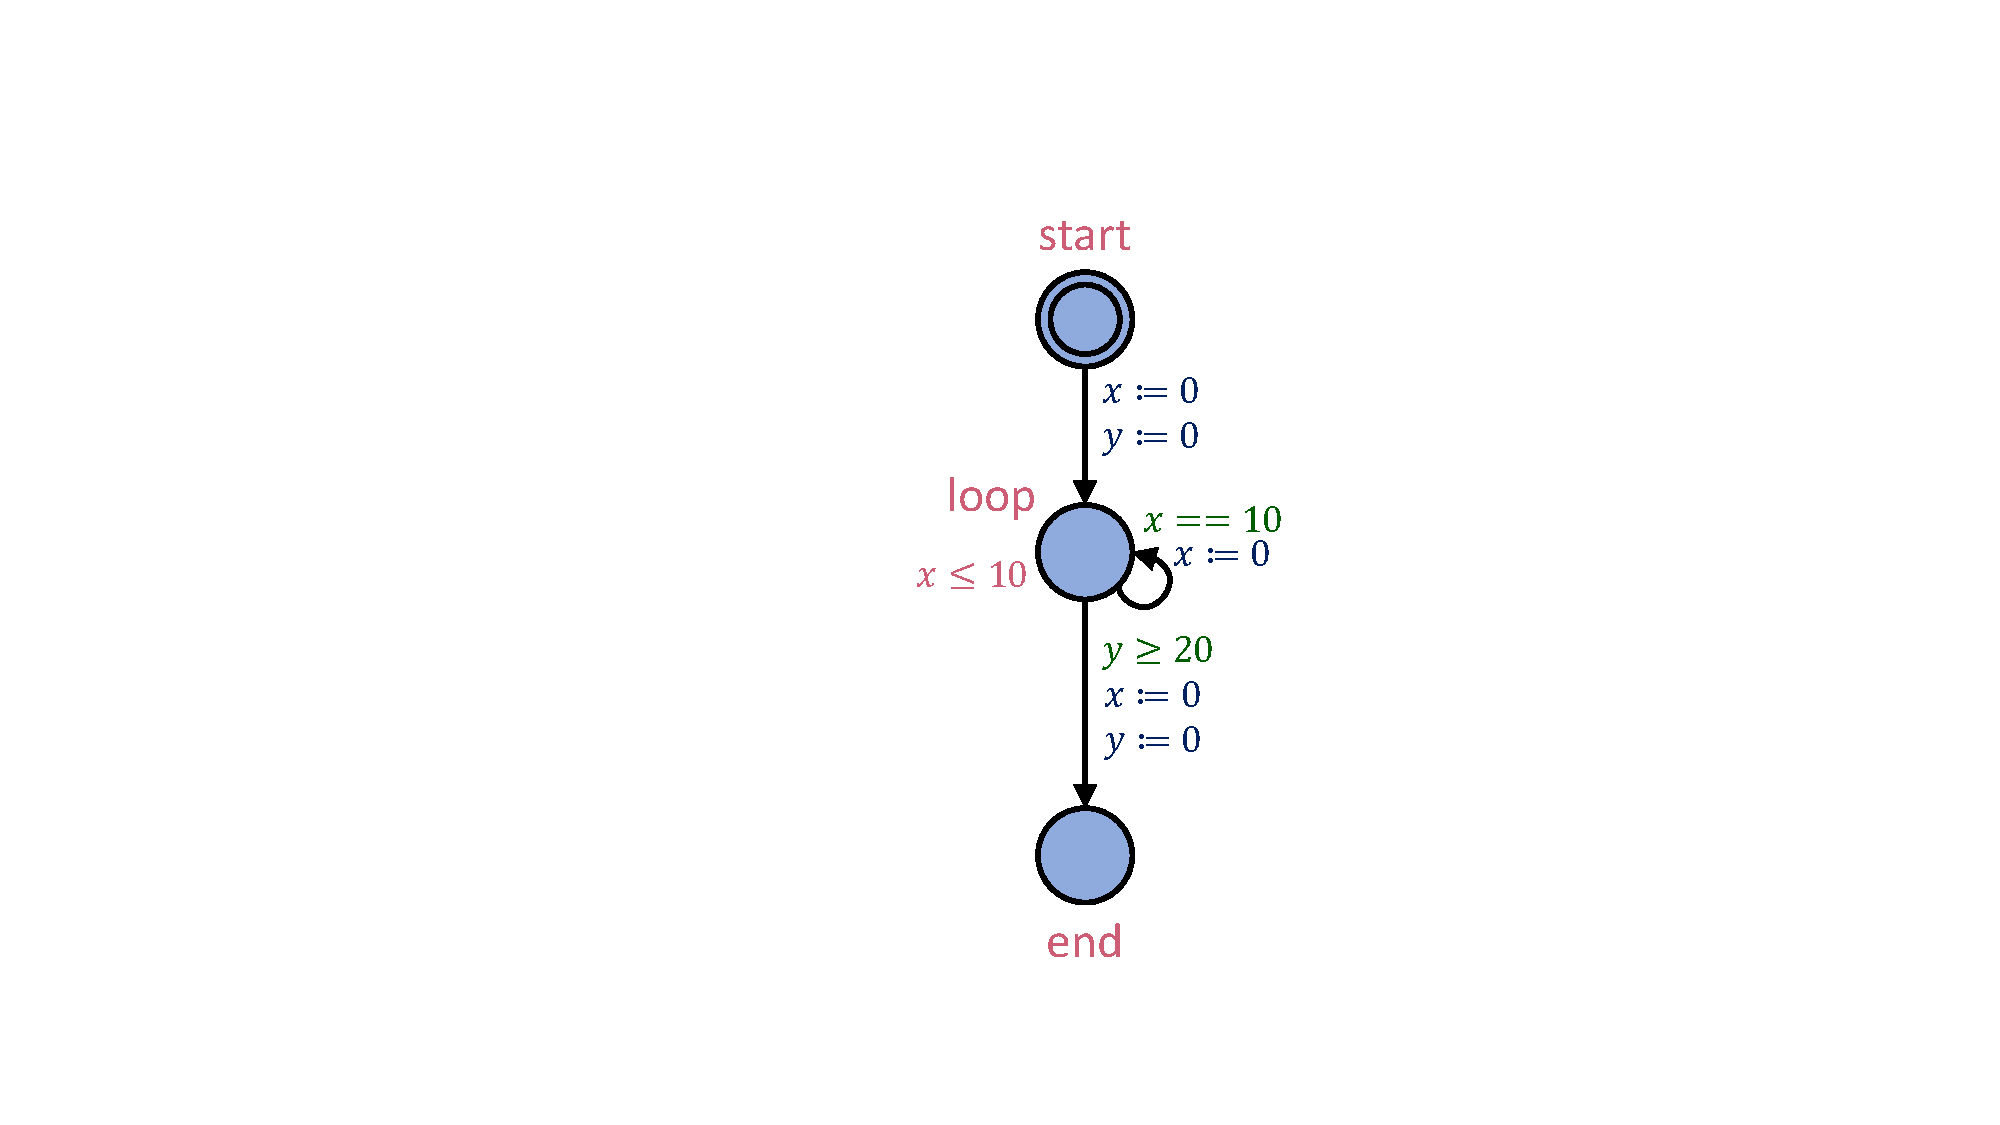
\includegraphics [width=\textwidth]{include/figures/loop_example_original}%
		%\caption{Example of a timed automaton}
		\label{fig:loopinfinite}
	\end{minipage}%
	%	%
	\begin{minipage}[c] {0.7\linewidth}%
		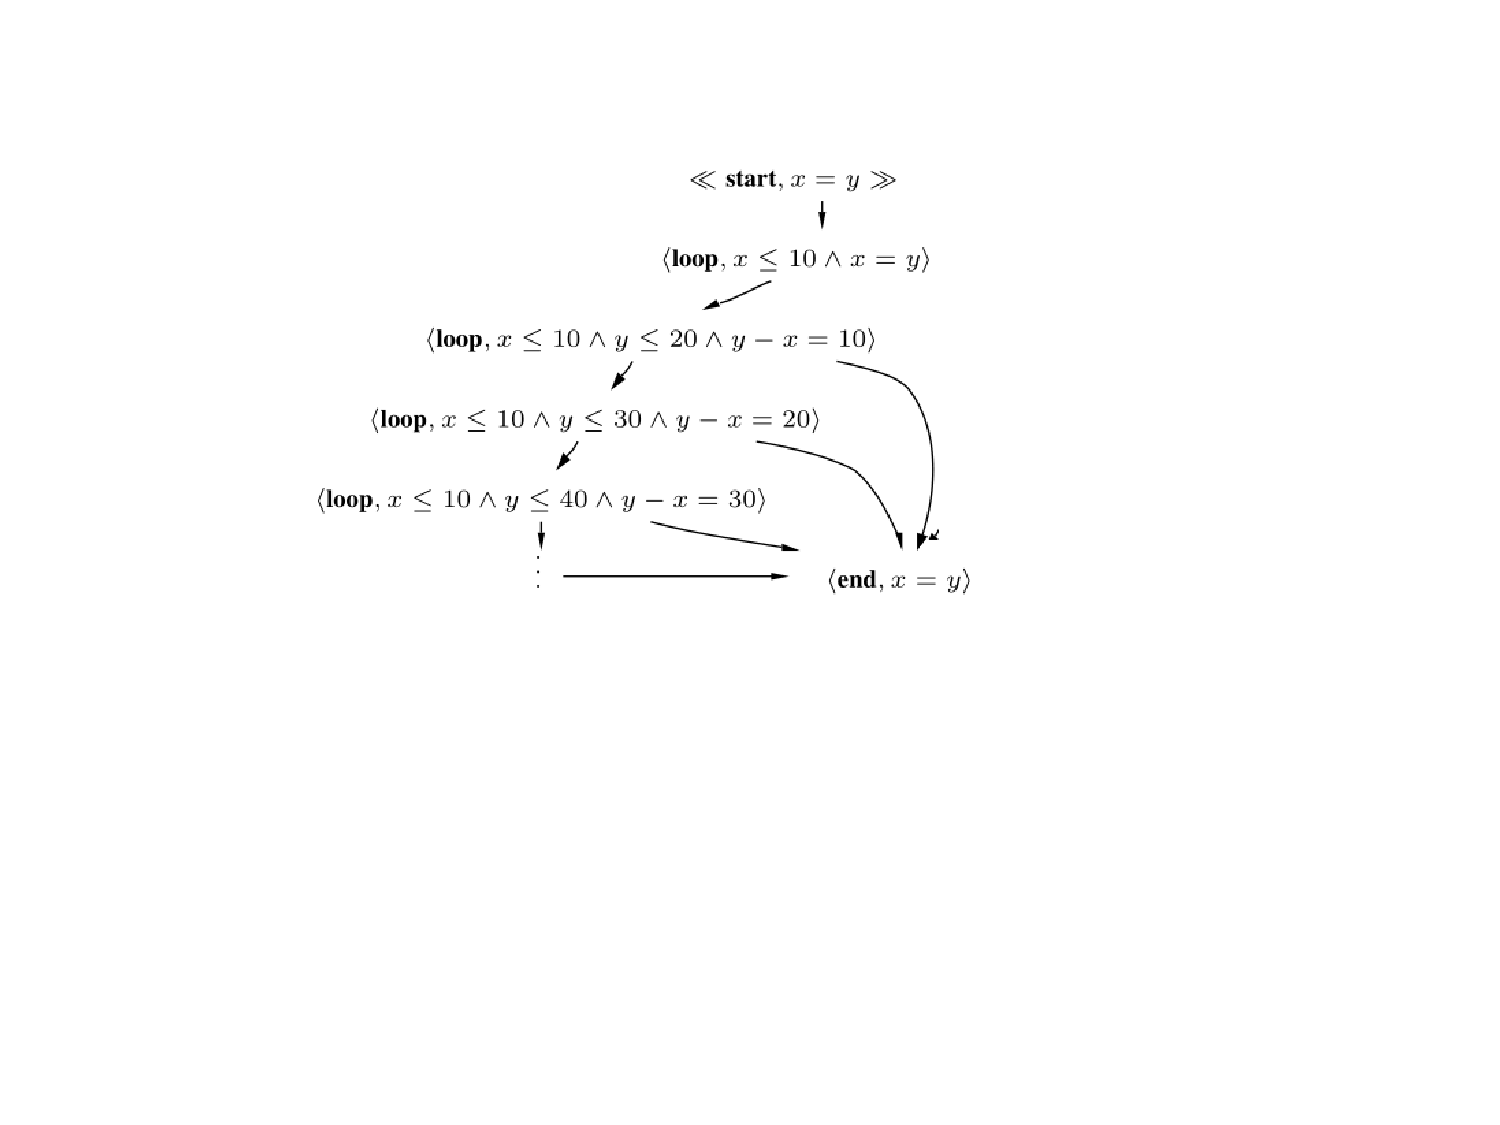
\includegraphics [width=\textwidth] {include/figures/loop_original_zonegraph}%TODO: ezt majd még vektorosítani
		%		\vspace*{4pt}%
		%		\caption{Timed automaton}
		\label{fig:loopinfinitegraph}
	\end{minipage}
	\caption{Timed automaton with infinite zone graph}
\end{figure} 

Unfortunately the described graph can possibly be infinite. Consider for example the automaton from \cite{bengtsson2004timed} on Figure \ref{fig:loopinfinite}. The only difference between this automaton and the one on figure \ref{fig:loopfinite}, is that in this automaton the transition represented by the loop edge only resets $x$, but not $y$.

\begin{example}
Constructing the zone graph of this automaton starts similarly, with the nodes $\langle start, x=y \rangle$ and $\langle loop, x=y \wedge x<10 \rangle$, where only the loop-transition is enabled.

This time the transition only resets $x$ resulting in $\langle loop, x=0 \wedge y=10 \rangle$. Because of the invariant, only 10 units of delay is enabled, resulting in the node $\langle loop, x \leq 10 \wedge y \leq 20 \wedge y-x=10 \rangle$.

From this node, both transitions are enabled. The loop transition increases the difference between $x$ and $y$ yielding the new node $\langle loop, x \leq 10 \wedge y \leq 30 \wedge y-x=20 \rangle$, while the other transition resets both clocks, resulting in the new node $\langle end, x=y \rangle$.

As we take the new node containing the location $loop$, and apply the loop transition over and over, a new node is always constructed with the difference growing. On the other hand, the other transition always results in $\langle end, x=y \rangle$.

Hence the (infinite) zone graph on Figure \ref{fig:loopinfinitegraph}.

\end{example}
	
In order for the zone graph to be finite, a concept called \emph{normalization} is introduced in \cite{bengtsson2004timed}.
Let $k(c)$ denote the greatest value to which clock $c$ is compared in the automaton.
For any valuations $v$ such that $v(c)>k(c)$ for some $c$, each constraint in the form $c > n$ is satisfied, and each constraint in the form $c = n$ or $c < n$ is unsatisfied, thus the interval $(k(c),\infty)$ can be used as one abstract value for $c$. 

Normalization is performed on $z^\uparrow$ (before inclusion is checked) in two steps. The first is removing all constraints of the form $x < m, x \leq m, x-y <m, x-y\leq m$ where $m>k(x)$ (so that $x$ doesn't have an upper bound), and the second is replacing constraints of the form $x > m, x \geq m, x-y >m, x-y\geq m$ where $m>k(x)$ by $x > k(x), x \geq k(x), x-y >k(x), x-y\geq k(x)$ respectively (to define the new lower bounds).

\begin{example}
In the automaton depicted on Figure \ref{fig:loopinfinite}, $k(y)=20$ (and $k(x)=10$). This means the exact value of $y$ doesn't really matter, as long as it is greater than 20 - the automaton will behave the exact same way if it is between 30 and 40, or if it is between 40 and 50. %We can combine the zones where $y$ is greater than 20 (and the value of $x$ is the same) into the zone $ x \leq 10 \wedge y>20 \wedge y-x>20$.
If we take this into consideration when constructing the zone graph, the zone  $x \leq 10 \wedge y-x=30$ can be normalized. In this zone, $y \geq 30 > k(y)=20$, but $x \leq k(x)$. This means we only have to consider constraints bounding $y$.
Implicitely $y \leq 40$ and $y-x \leq 30$. These constraints have to be removed from the zone. Similarly, $y \geq 30$ and $y-x \geq 30$ have to be replaced by $y \geq 20$ and $y-x \geq 20$. The resulting zone is $x \leq 10 \wedge y \geq 20 \wedge y-x \geq 20$. If we replace the original zone  $x \leq 10 \wedge y-x=30$ by this zone, and continue constructing the zone graph, the resulting graph, depicted on Figure \ref{fig:looprealgraph}.

\end{example}

\begin{figure}
	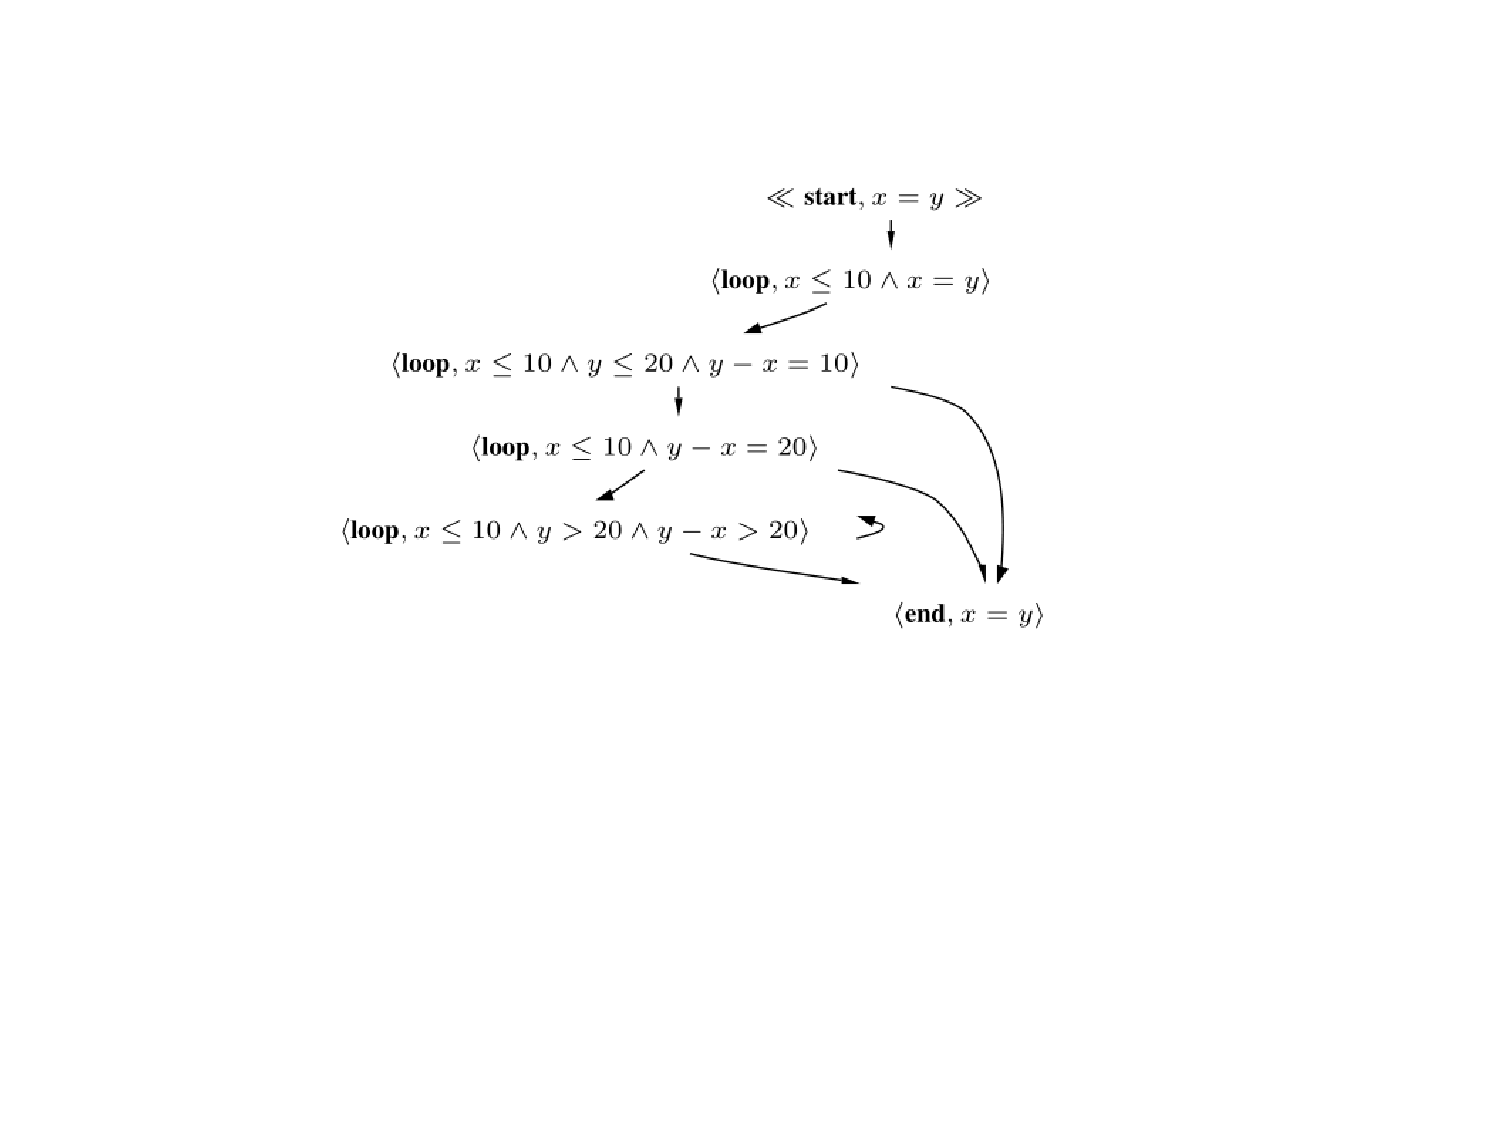
\includegraphics [width=0.7\textwidth] {include/figures/loop_real_zonegraph}%TODO: ezt majd még vektorosítani
	%		\vspace*{4pt}%
	%		\caption{Timed automaton}
	\label{fig:looprealgraph}
\end{figure}

Using normalization the zone graph is finite, but unreachable states may appear in it. If the automaton doesn't have any guard or invarint of the form $c_1 - c_2 < n$, the reachability of the location in question will be answered correctly. Otherwise, the algorithm may terminate with a false positive result.

\todo{Példa}

The operation \emph{split} \cite{bengtsson2004timed} is introduced to eliminate such states. Instead of
normalizing the complete zone, it is first split along the difference constraints,
then each subzone is normalized, and finally the initially satisfied constraints are reapplied to each zone. If the result is a set of zones, then multiple new nodes have to be introduced to the zone graph. Applying split results in a zone
graph, that is a correct and finite representation of the state space.


\todo{magyarázóábra, példa, stb}

%\emph{Example:}
%Fischer's protocol assures mutual exclusion by bounding the execution
%times of the instructions. It can be applied to a number of processes accessing a
%shared variable. Fig. \ref{fig:fischer}  shows the operation of a process.
%The location \emph{critical} indicates that the process is in the critical
%section. The value of the shared variable $id$ ranges between 0 and $n$,
%where $n$ denotes the number of processes. The model also contains a 
%clock variable $x_i$ for each process where $i \in \{1 \ldots n\}$ denotes the
%identifier of the process. The constant $k$ is a parameter of the automaton.

%\begin{figure}
%	\centering
%	\begin{minipage}[c] {0.575\linewidth}%
%		\vspace*{1pt}%
%		\includegraphics [width=\textwidth]{fischer_vertical}%
%		\caption{Fischer's protocol}
%		\label{fig:fischer}
%	\end{minipage}%
%	%
%	\begin{minipage}[c] {0.425\linewidth}%
%		\includegraphics [width=\textwidth] {fischer_product_1}%
%		\vspace*{4pt}%
%		\caption{Timed automaton}
%		\label{fig:fischer_product}
%	\end{minipage}
%\end{figure}  

%\todo{figure}

%The mutual exclusion property would suggest that at any given time
%at most one of the processes is in the \emph{critical} location. In order to
%check the given property we must construct a timed automaton that models the
%operation of a given number of processes.

%As our definition of timed automaton only allows clock variables in the system,
%everything else must be encoded in the location.
%  First, to represent the
% location of all processes simultaneously, we construct a product automaton
% containing one location for each of the $4^n$ -- not necessarily reachable --
% possible combinations. 
% %For example, the initial location will be \{sleeping, sleeping, \ldots \} with
% % an outgoing edge to each location containing a combination of $n-1$ sleeping
% % plus one request label and the corresponding invariant. 
% The $id$ variable can
% be encoded in the locations the exact same way.
% The edges, invariants, etc. should be created approriately.
% Each location of the result automaton will be denoted by a combination of
% the four original locations and a number representing $id$'s value. 
%To
%demonstrate, Fig.
%\ref{fig:fischer_product} shows the reachable locations of the product automaton
%of Fischer's protocol where $n=1$. The names of the locations refer to the original locations of the process, the number denotes the value of the variable $id$.


\section{CEGAR}

%\begin{figure}[b]
%	\centering
%	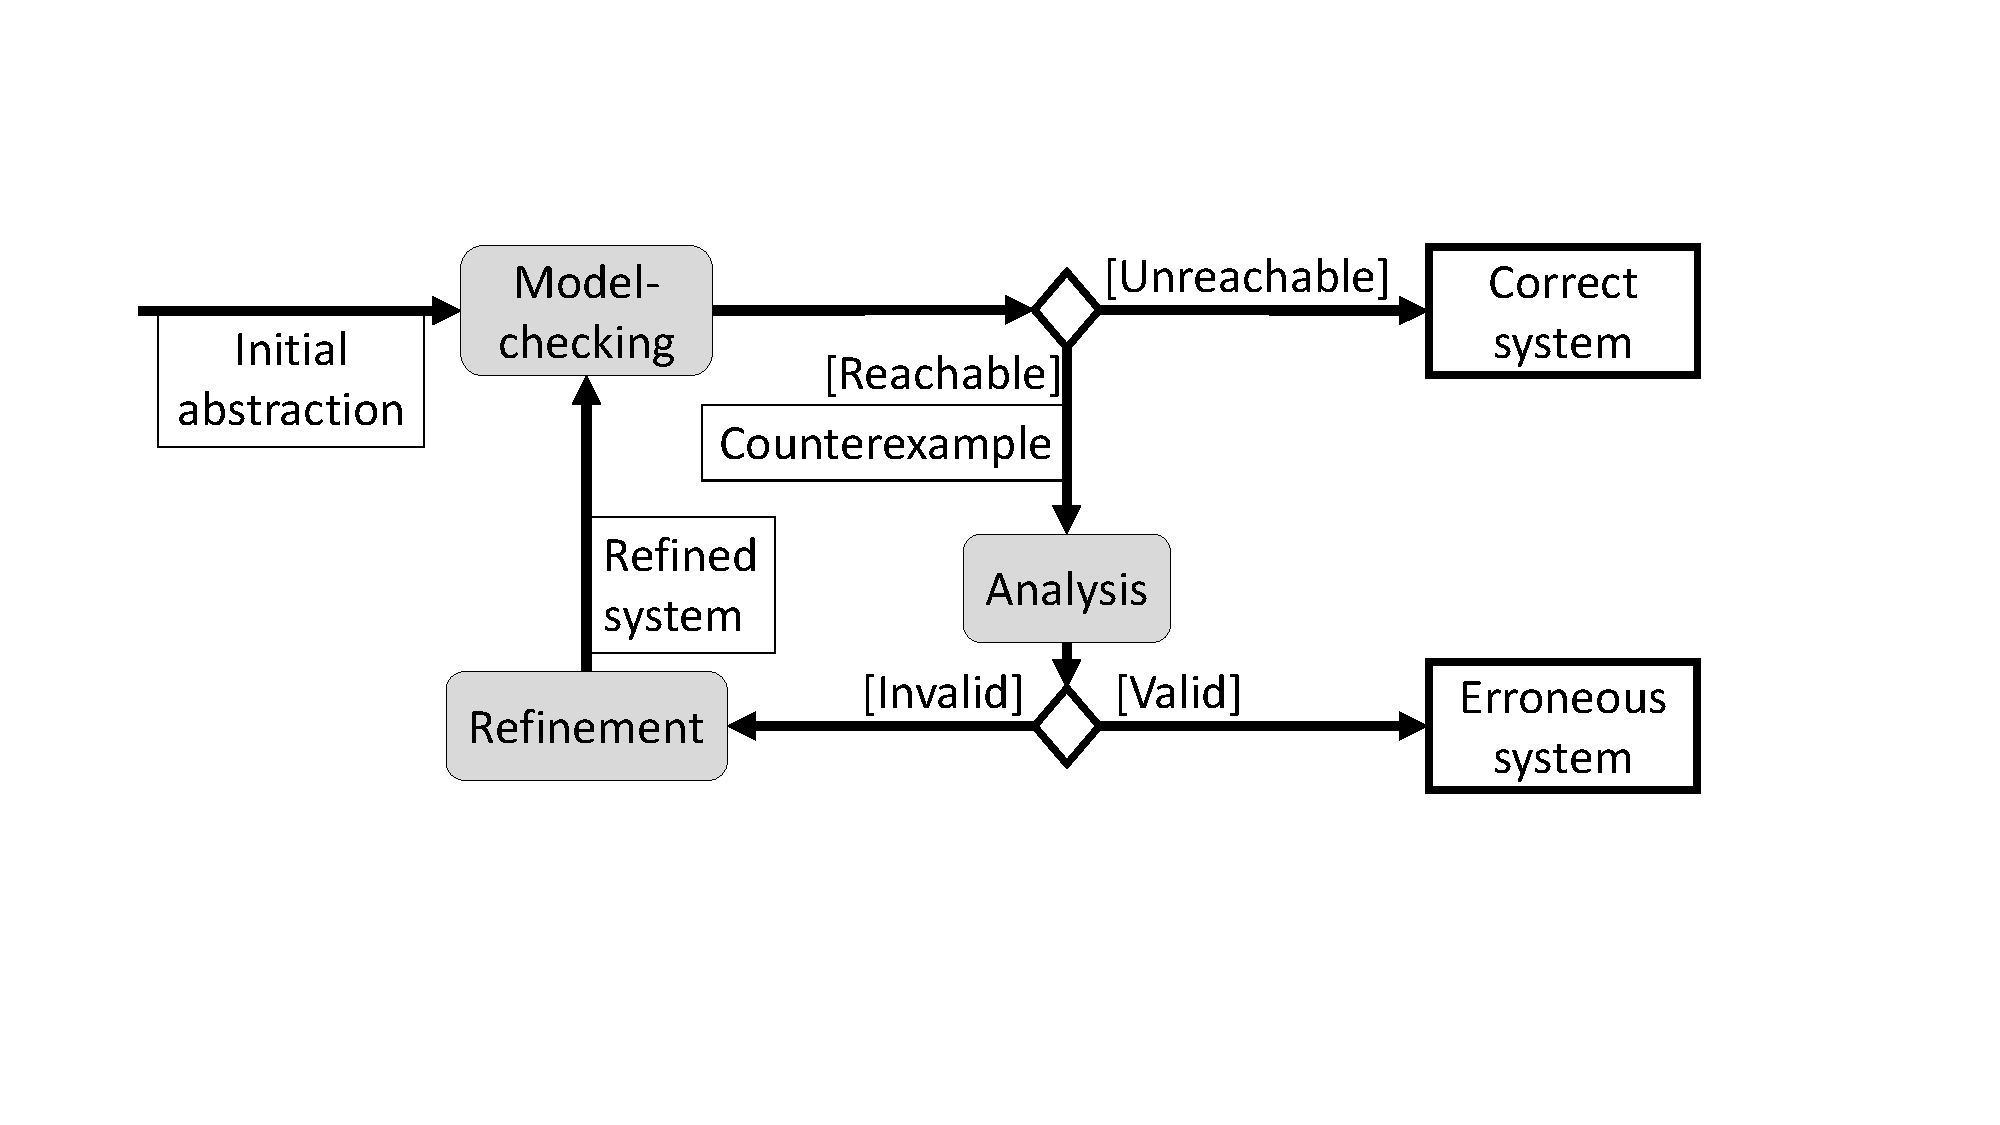
\includegraphics [width=3.5in] {cegar_flow_black}
%	\caption{Counterexample guided abstraction refinement}
%	\label{fig:cegar}
%\end{figure}

\todo{ábra}

The CEGAR approach introduced in \cite{clarke2003counterexample} makes
abstraction refinement a key part of model checking. The idea is illustrated on
Fig. \ref{fig:cegar}.

First, an abstract system is constructed. The key idea behind abstraction is
that the state space of the abstract system overapproximates that of the original
one. 
Model checking is performed on this abstract model. If the target state is
unreachable in the abstract model, it is unreachable in the original model
as well. Otherwise the model-checker produces a counterexample -- a run where the
system reaches the target state. In our case the counterexample is a sequence of
transitions -- i.e., a trace. Overapproximation brings such behaviors to the system that are not feasible in the original one. Because of this, the counterexample may not be a valid trace in the real system, so it has to be investigated.
If it turns
out to be a feasible counterexample, the target state is reachable. Otherwise
the abstract system has to be refined. The goal of the refinement is to modify the abstract
system so that it remains an abstraction of the original one, but the spurious
counterexample is eliminated.  Model checking is performed on the
refined system, and the CEGAR-loop starts over. 

The algorithm terminates when no more
counterexample is found or when a feasible trace is
given leading to the erroneous state.